\documentclass{standalone}
\usepackage{tikz}
\usetikzlibrary{positioning}
\begin{document}
    % original
        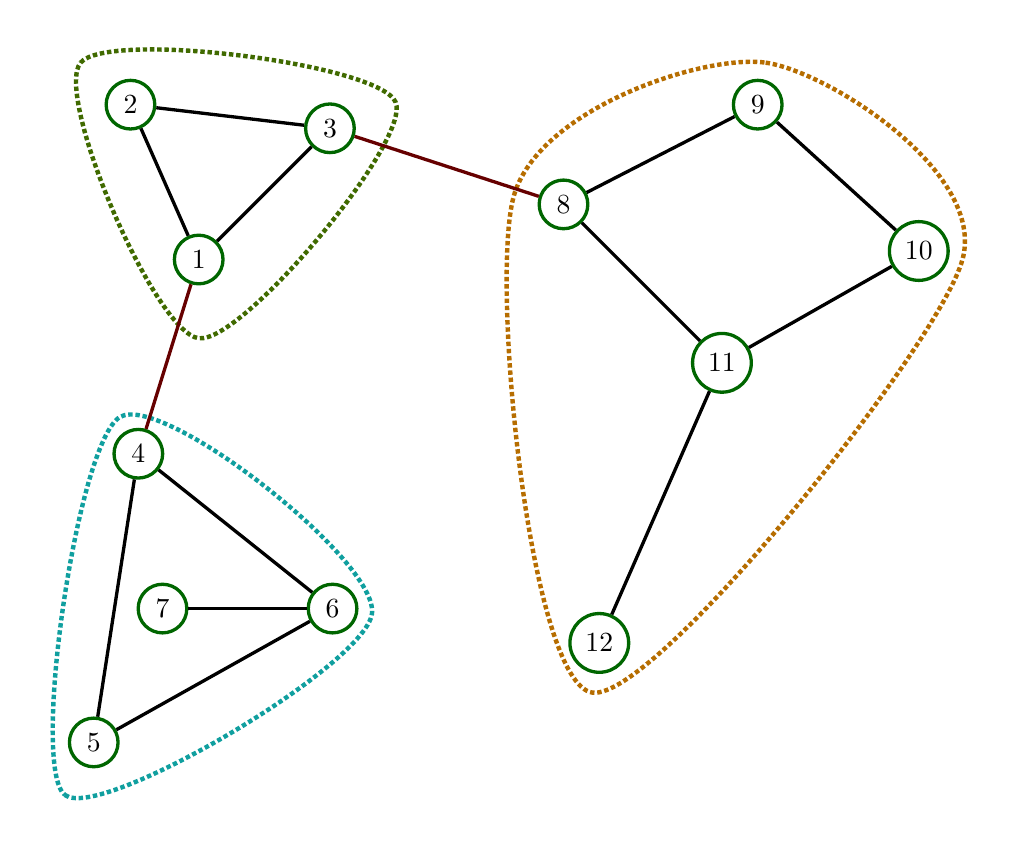
\begin{tikzpicture}[
        core_node/.style={circle, draw=black!60!green, very thick, minimum size=4mm},  %fill=black!15!green,
        copy_node/.style={rectangle, draw=blue!60, fill=blue!5, very thick, minimum size=5mm},
        ]
            % areas
            \draw [color={rgb:red,2;green,4;yellow,1;black,5}, ultra thick,  densely dotted] plot [mark=none, smooth cycle] coordinates {(0,-1)  (-1.5,2.5)  (2.5,2) };
            \draw[color={rgb:red,1;cyan,10;black,5}, ultra thick,  densely dotted] plot [mark=none, smooth cycle] coordinates {(-1,-2)  (-1.7,-6.8)  (2.2,-4.5) };
            \draw[color={rgb:red,4;green,2;yellow,1}, ultra thick,  densely dotted] plot [mark=none, smooth cycle] coordinates {(4,0.8)  (7.2,2.5)  (9.7,0) (5, -5.5)};
        
            % transmission
            \node[core_node]    (core_1)                                               {1};
            \node[core_node]    (core_2)   [above left  = 15mm and 4mm of core_1]      {2};
            \node[core_node]    (core_3)   [above right = 12mm and 12mm of core_1]     {3};
            % distribution 1
            \node[core_node]    (core_4)   [below left  = 20mm and 3mm of core_1]      {4};
            \node[core_node]    (core_5)   [below left  = 32mm and 1mm of core_4]      {5};
            \node[core_node]    (core_6)   [below right = 15mm and 20mm of core_4]     {6};
            \node[core_node]    (core_7)   [left        = 15mm of core_6]              {7};
            % distribution 2
            \node[core_node]    (core_8)   [below right  = 5mm and 25 mm of core_3]    {8};
            \node[core_node]    (core_9)   [above right  = 8mm and 20mm of core_8]     {9};
            \node[core_node]    (core_10)  [below right  = 0.8mm and 40mm of core_8]   {10};
            \node[core_node]    (core_11)  [below right  = 15mm and 15mm of core_8]    {11};
            \node[core_node]    (core_12)  [below left  = 30mm and 10mm of core_11]    {12};
            
            % Lines
            \draw[black, very thick, -] (core_1) -- (core_2);
            \draw[black, very thick, -] (core_2) -- (core_3);
            \draw[black, very thick, -] (core_3) -- (core_1);
            \draw[black, very thick, -] (core_4) -- (core_5);
            \draw[black, very thick, -] (core_5) -- (core_6);
            \draw[black, very thick, -] (core_6) -- (core_7);
            \draw[black, very thick, -] (core_6) -- (core_4);
            \draw[black, very thick, -] (core_8) -- (core_9);
            \draw[black, very thick, -] (core_9) -- (core_10);
            \draw[black, very thick, -] (core_10) -- (core_11);
            \draw[black, very thick, -] (core_11) -- (core_12);
            \draw[black, very thick, -] (core_11) -- (core_8);
            
            % connection
            \draw[color=black!60!red, very thick,-] (core_1) -- (core_4);
            \draw[color=black!60!red, very thick,-] (core_3) -- (core_8);
        \end{tikzpicture}
\end{document}